% -*- root: ../../main.tex -*-
%!TEX root = ../../main.tex
% this file is called up by main.tex
% content in this file will be fed into the main document
% vim:textwidth=80 fo=cqt

\subsection{The transfer operator and its model form}
In a classical system identification  task, the discrete-time transfer functions
for the systems  under consideration need to be  determined. These discrete-time
transfer functions are  based on Z-transforms in the  frequency domain. However,
for the purpose of working in time-domain, an analogous linear operator~$q$ that
performs a  forward shift on  its input \ie~$  {q u[k] \longmapsto  u[k+1]} $.
Similarly, applying the  backward shift operator~$ q^{-1} $  on the input yields
its value at the previous time-step \ie~$ {q^{-1} u[k] \longmapsto u[k-1]}$.


In a generic  \gls{lti} system wherein measurements are corrupted  by noise, The
system  dynamics are  represented by  the transfer  operator~$G(q)$\footnote{The
term  transfer operator  in the  time domain  mathematically corresponds  to the
term  transfer  function  in  the  frequency  domain.  Mathematically,~${G(q)  =
G(z)\bigr\rvert_{\mathrlap{z=q}}}$.}  that  acts  on the  applied  input~$u[k]$,
whereas the  noise dynamics are  represented by the  disturbance operator~$H(q)$
that acts to filter (or shape) an assumed white noise input~$e[k]$.

Assuming linearity and time-invariance throughout, the overall output can be
written as the linear combination
\begin{equation}\label{eq:outputwithsysandnoise}
    % \SwapAboveDisplaySkip
    y[k] = G(q)u[k] + H(q)e[k]
\end{equation}
where ${G(q) = \frac{B(q)}{A(q)}}$ and ${H(q) = \frac{C(q)}{D(q)}}$ are the transfer
operators describing the dynamics of the system and disturbance respectively.

${A(q), B(q), C(q) \text{ and } D(q)}$ are rational polynomials in~$q$. The two transfer
operators~$G(q)$ and $H(q)$ can be represented by
\begin{align}
    G(q) &= q^{-n_k}\frac{b_1q^{-1} + \dots  + b_{n_b}q^{-{n_b}}}{1 + a_1q^{-1} + \dots  + a_{n_a}q^{-{n_a}}} \\
    H(q) &= q^{-n_l}\frac{c_1q^{-1} + \dots  + c_{n_c}q^{-{n_c}}}{1 + d_1q^{-1} + \dots  + d_{n_d}q^{-{n_d}}}
\end{align}
where ${(n_k,n_l)}$ represent  the number of transport  delay samples, $(n_b,n_c)$
the number  of feedforward coefficients  and ${(n_a,n_d)}$, the number  of feedback
coefficients in $G(q)$ and $H(q)$ respectively.


% In  this  system  identification  task  at hand,  the  output  measurements  are
% collected from a  \emph{noise-free} simulation of the \gls{p2d}  model \ie~the
% disturbance transfer operator in \cref{eq:outputwithsysandnoise} is zero
% \begin{align}
%     y[k] &= G(q)u[k] + \cancelto{0}{H(q)}e[k]
% \shortintertext{Hence, the time-domain output  reduces  to}
% y[k] &= G(q)u[k] \label{eq:outputwithsysonly}
% \end{align}

Thus, the system identification task becomes one that of estimating
\begin{enumerate}
    \item The number of transport delay samples~$n_k$.
    \item The number of feedforward coefficients (zeros)~$n_b$.
    \item The zeros themselves~${b_1, b_2, \dots b_{n_b}}$.
    \item The number of feedback coefficients (poles)~$n_a$.
    \item The pole locations~${a_1, a_2 \dots a_{n_a}}$.
    \item The coefficients of the noise filter~$H(q)$\footnote{In the \gls{armax} estimation of non-linear dynamics, the
noise-filter is capable of returning non-zero coefficients even if the
identification data set is obtained from a \gls{noise-free} simulation of the
\gls{p2d} model as is the case here. However, as a first-order approximation, in
the interest of simplicity and considering that this work serves as an
introduction to the application of system identification to \glspl{spm}, this thesis author errs on
the side of making the linearity assumption, which is valid only for low
C-rates, whilst acknowledging that this
limitation could be relaxed by incorporating the coefficients of the
noise-filter~$H(q)$ in the future. For the rest of this work, only the
coefficients of the linear plant dynamics~$G(q)$ are estimated.}.
\end{enumerate}
for  each  of  the  two  transfer operators~$G_1(q)$  and  $G_2(q)$  \ie~the
electrolyte  time-evolution subsystems  in the  negative and  positive electrode
region respectively.

\subsection{Estimation of transport delay}

The transport delay~$n_k$ can be estimated visually by inspecting the step
response of the systems under consideration.

In \cref{fig:linearity},   step  inputs   of   ${I_1   =  \SI{60}{\ampere},   I_2
=    \SI{12}{\ampere},}$   and    ${I_3   =    \SI{36}{\ampere}}$   were    applied
to    the   two    subsystems.    Inspecting   closely    all   the    responses
\ie~$\widetilde{Q}_{\text{e,n}_1},    \widetilde{Q}_{\text{e,n}_2}   $   and
$\widetilde{Q}_{\text{e,n}_3}$    in    the     negative    electrode    region,
and    $\widetilde{Q}_{\text{e,p}_1},    \widetilde{Q}_{\text{e,p}_2}   $    and
$\widetilde{Q}_{\text{e,p}_3}$  in the  positive electrode  region, it  is clear
that all these outputs start exactly at  zero. Therefore, there is no delay term
to be considered for the transfer operators \ie~${n_k = 0}$ for both subsystems.

\subsection{Choice of model structure}\label{subsec:modelstrucchoice}

Among      the      transfer-function       model      structures      mentioned
in \cref{subsec:parametric}, the \gls{arx} model  structure is too simplistic to
consider. Despite  the fact that  its numerical computation involves  only basic
linear algebra operations,  that can be efficiently handled  on modern computing
systems, it  is considered to produce  poor estimates of the  system's poles and
zeros. In the absence of contributions from the noise-term, the all-encompassing
model structure used by the Box-Jenkins approach is deemed to be unnecessary for
the  problem  at hand.  Therefore,  the  two  model structures  considered  were
\gls{armax} and \gls{oe} for the coefficient determination.

\subsection{Starting guesses for coefficient orders}\label{subsec:initguesscoefforder}

At first, the training profile of \cref{fig:sysidtrainingcurrent} is de-biased
(through mean removal) and applied as the input current profile in a \gls{p2d}
simulation beginning at \SI{50}{\percent}~\gls{soc}. The outputs of this
simulation are suitably post-processed as per the following sequence of steps.
\begin{enumerate}
    \item The concentrations solved at various node locations within each
        electrode are numerically integrated over the corresponding electrode
        thicknesses using trapezoidal rule.
    \item The resulting integral value is multiplied with the porosity of the
        corresponding electrode region to obtain
        $Q_{\text{e,n}_\text{train}}(t)$ and~$Q_{\text{e,p}_\text{train}}(t)$.
    \item These quantities are then de-biased by subtracting their initial
        values to obtain $\widetilde{Q}_{\text{e,n}_\text{train}}(t)$
        and~$\widetilde{Q}_{\text{e,p}_\text{train}}(t)$.
\end{enumerate}

The        same        procedure        is        repeated        for        the
validation       current      profile       of \cref{fig:sysidvalidationcurrent}
to         obtain         $\widetilde{Q}_{\text{e,n}_\text{val}}(t)$         and~$\widetilde{Q}_{\text{e,n}_\text{val}}(t)$.  These data  sets are  used for  all
subsequent sub-tasks involved in this system identification exercise.

In  order to  reduce  the search  window for  the  coefficient determination  in
the  parametric transfer  function methods,  the hand-estimation  of coefficient
order  through non-parametric  methods may  be performed.  This coarse  estimate
can  act as  a  feeder to  help  in  the faster  convergence  of the  non-linear
optimisation algorithms  used in the parametric  methods. In this case,  a basic
spectral analysis  using a Hanning  window implemented using the  MATLAB command
\texttt{spa.m} is applied to the time-domain data to transform it into frequency
response data.

\begin{figure}[!htb]
    \centering
    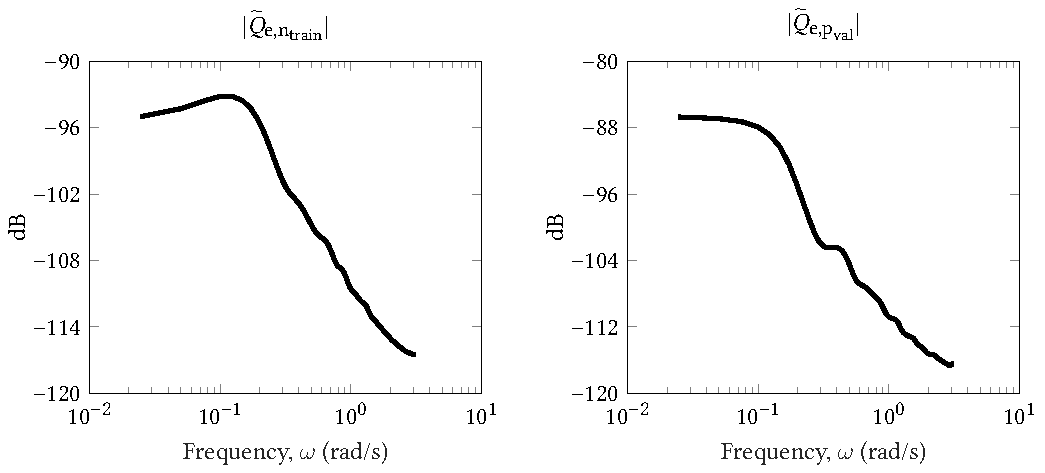
\includegraphics[width=\textwidth]{bode_mag.pdf}
    \caption[Bode plots of the electrolyte time-evolution sub-systems]{%
        Bode plots showing the  estimated frequency response  for the
        two  subsystems under  consideration.  The frequency  response data  was
        obtained  through a spectral  analysis \ie~by computing  the ratios  of
        spectra of the de-biased input  and output sequences. The sequences were
        smoothed using a Hanning window before computing the ratio.
    }%
    \label{fig:initialbodemag}
\end{figure}

\Cref{fig:initialbodemag}  shows  the  Bode  plots  of  the  frequency response
to the training set in the negative electrode (left column) and positive
electrode (right column) regions of the cell. It is important to note that these
Bode diagrams obtained by such non-parametric methods only represent  an
approximation of the  physical dynamics intended to help in initial estimates of
the system behaviour. Some preliminary understanding of the  various
characteristics of the system can be gleaned from these Bode diagrams.  The
first visually striking feature is the similarity  in the  general shape of the
approximate frequency characteristics in  the negative  and positive electrode
regions, both in the magnitude response and in the phase response. This confirms
the author's assumptions of equal `complexity' in the symbolic  regression
search discussed in \cref{subsec:symbolicreg}.  This is also  congruent with
the physical  behaviour of  the electrolyte  in these  two regions.

\subsubsection*{Finite DC gain}
By visual  extension of  the frequency responses  towards lower  frequencies, it
is  clear  that  the  DC  gains  of  both  the  systems  are  finite  and  below
unity.  This  behaviour  can  clearly  be  seen  in  the  time-domain  responses
of \cref{fig:linearity}.  For  the plotted  time-horizon,  this  effect is  most
visible for the case of the \SI{12}{\ampere} constant current input, wherein the
responses of both regions settle to a finite value after an initial transient.
Finally, the finiteness  of the DC gain  helps to narrow down  the search window
for the parametric model structures. In particular, this fact indicates that the
model structures to be trialled must not  have any integrator terms (or poles at
the origin of the complex plane).


% There is \approx\SI{10}{\decibel} variability in  the low frequency gain between
% the two Bode  plots in \cref{fig:initialbodemag}. This can be  attributed to the
% following  factors. A  compromise with  the spectral  estimation method  is that
% using a higher number of frequency bins  results in lower resolution per bin and
% vice-versa. By  varying the number  of frequency bins  and focusing on  the low
% frequency range, the resolution of the DC  gain can be improved. The rest of the
% variability can  be attributed to the  fact that the training  and test profiles
% behave differently and do not excite the same dynamics. In particular, the swept
% frequency cosine (chirp) signal in the training set was specifically designed to
% draw out  the low frequency  dynamics with a  high fidelity. Finally,  the small
% range of variation in the DC gain could also be due to the intrinsic small-scale
% variations of  the electrolyte  behaviour in  these two  regions. Although  on a
% macroscopic frequency scale the two regions behave similarly, the differences in
% electrode thicknesses and porosities could contribute to the small difference in
% the  DC gain.  This  helps  to confirm  that  two \emph{non-identical}  transfer
% functions are being sought for --- one for each electrode region.

\subsubsection*{Resonance and model order}

First  order  transfer   functions  do  not  exhibit   characteristic  peaks  or
resonances  in  their  frequency  responses.  However,  for  the  Bode
magnitude plots  in \cref{fig:initialbodemag},   a   pronounced   resonance   around
\SI{0.15}{\radian\per\second} is observable. This has  an enormous impact --- it
presents  an important  clue  that the  first  order time-evolution  \glspl{ode}
of \cref{eq:negliionmolesquadratic}   and \cref{eq:posliionmolesquadratic}   are
inadequate to represent the system dynamics.

% An apparent  contradiction to  the first-order inadequacy  claim stems  from the
% Bode plot  on the  right hand side  in \cref{fig:initialbodemag}. In  this case,
% there are no resonances in the  magnitude response indicating that a first order
% model description is sufficient. However, a vital aspect to be noted here is the
% nature of the  validation current profile when compared to  that of the training
% current profile.  The coarse  frequency response data  obtained by  the spectral
% method is sensitive to the actual  input sequence employed. From systems theory,
% the  resonances at  a frequency  occur  due to  the presence  of lightly  damped
% complex conjugate poles at that frequency. The periodic \gls{rgs} was explicitly
% designed in the  training set and is  however absent in the  validation set. The
% unique characteristics  of the validation  set and its influence  on coefficient
% order is discussed next.

% As per  the arguments presented  in the  discussions so far, there  exists an
% implicit constraint that  the behaviour of the time-evolution  subsystems in the
% two electrode  regions are  expected to be  of similar  `complexity'. Therefore,
% based  on the  presence of  the resonance  in the  Bode magnitude  plot for  the
% response to  training profile,  it has  to be concluded that the two subsystems
% are \emph{at-least} of second order.

\subsubsection*{Estimation of number of poles and zeros}

The  high-frequency  roll-off  in  the   slopes  of  the  Bode  magnitude  plots
in  \cref{fig:initialbodemag}  provide clues  on  the  number  of poles  in  the
system.  The  corner frequency~$\omega_\text{c}$  in  both  cases appear  to  be
around~\SI{0.15}{\radian\per\second}. The  high-frequency slope of  both systems
is \approx\SI{20}{\decibel}  per decade, which  implies that they  have at-least
one more  pole than  the number  of zeros  if using  a continuous  time transfer
function. For  the corresponding z-domain  transfer function, this  implies $n_a
\ge n_b$. Looking at the phase plot of the two electrode regions, it can be
hypothesised that there exists at-least one zero in these  continuous-time
systems around the \SIrange{0.3}{0.4}{\radian\per\second} frequency range. The
discrete-time sampling process adds an additional zero to the system.

% In the  aspect of estimating the  number and locations of  zeros, the validation
% profile outshines  the training profile. While  the Bode plot obtained  with the
% training profile  does not indicate  the presence of  zeros in the  systems, the
% plateau in \SIrange{0.3}{0.4}{\hertz} range for  the Bode plot of the validation
% profile clearly contradicts this.

Based on this preliminary  analysis, the estimates are $n_k = 0,  n_b \ge 2, n_a
\ge 3$.  Only asymptotic approximations  to corner frequencies can  be estimated
from the  Bode plots. Furthermore, the  estimated locations are not  used in the
parametric system identification algorithms and  is of much less importance than
the  model order  estimates.  With this  initial  understanding, the  parametric
system identification procedure is carried out.

\subsection{Refinement of coefficient orders using deterministic criteria}\label{subsec:refinementofcoefforder}

The initial estimate  of coefficient orders in \cref{subsec:initguesscoefforder}
was performed  based only on  a visual inspection  of the Bode  magnitude plots.
Owing to  the fact that  the frequency  response data is  the result of  a crude
ratio of  spectra, there is a  high probability of missing  vital information on
the number and locations of poles and zeros. Hence only a lower bound on the
coefficient orders are available until this point. Next, a set of deterministic
criteria is used to widen and refine the coefficient order range.


Although   the   \gls{arx}   structure   is  deemed   to   be   too   simplistic
(see \cref{subsec:modelstrucchoice}), owing to the fact that only linear algebra
operations are involved, as opposed  to numerical optimisation routines employed
in the  \gls{oe}, \gls{armax} and Box-Jenkins  structures, certain deterministic
criteria can  be incorporated  for coefficient order selection. This  can serve
as  a  refinement  of  the initial number of  coefficients guessed from the Bode
magnitude plots.

For any model structure used, its error can be defined as
\begin{align}
    % \SwapAboveDisplaySkip
    \varepsilon[k]      & = y[k] - \hat{y}_\text{m}[k] \label{eq:sysiderroronlyk}\\
    \shortintertext{where $y[k]$ are true measurements and}
    \hat{y}_\text{m}[k] & = G(q)u[k] \tag{\cref{eq:outputwithsysonly} revisited}
\end{align}
are the model outputs obtained by the assumed transfer operator~$G(q)$ (which is
to be determined).

The  number of  numerator  and denominator  coefficients in  $G(q)$  as well  as
their  values are  to  be determined.  This  set of  unknowns  can be  collected
into a  parameter vector~$\theta$.  Thus, as per  \cref{eq:sysiderroronlyk}, the
error  sequence  is  parametrised  by  $\theta$, and  its  notation  is  amended
to~$\varepsilon[k;\theta]$.

For  an  input-output  data  set  consisting of  $N$~samples,  a  generic  cost
function that may  be applied for all the four  model structures \viz{\gls{arx},
\gls{armax}, \gls{oe} and Box-Jenkins} is
\begin{align}
    V_N(\theta)  & = \sum_{k=1}^N L\left(\varepsilon\left[k;\theta\right]\right)
\shortintertext{where $L(\cdot)$ is a postive-valued scalar loss function.}
\intertext{In a typical system identification task, the sum of squares of the error sequence is  used as the typical loss function, thereby yielding}
    V_N(\theta)  & = \sum_{k=1}^N \varepsilon^2[k;\theta]\label{eq:nonlincostfcnsysid}
    \shortintertext{The vector~$\hat{\theta}$ that minimises this cost function is desired}
    \hat{\theta} & = \text{arg}\,\underset{\theta}{\text{min}} V_N(\theta)
\end{align}

For  the \gls{arx}  model structure, \cref{eq:nonlincostfcnsysid}  reduces to  a
standard quadratic optimisation  problem which may be  solved analytically using
least  squares  linear  algebra.  However,  for  robustness  against  estimation
bias,  instead of  the  standard \gls{ols}  estimates,  the \gls{iv}  estimation
method~\cite{Ljung1999} was used  for this model order  selection task. Applying
this to  the \gls{arx} model  structure, two deterministic model  order criteria
have been defined ---
\begin{enumerate*}[label=\emph{\alph*})]
    \item \gls{aic}, and
    \item \gls{mdl}~\cite{Ljung1999}.
\end{enumerate*}

In  the \gls{aic},  the  optimal  number of  parameters~$\hat{d}$ in  $\theta$
is  obtained   by  minimising   the  modified   log  likelihood   cost  function
\begin{equation}
    V_{N,\text{mod}}(\theta) =  \ln V_N(\theta)  + \frac{2  d}{N}, \quad N \gg d
\end{equation}
In the \gls{mdl} criterion, this cost function is modified to
\begin{equation}
    V_{N,\text{mod}}(\theta) =  V_N(\theta)\left(1 + \frac{d\, \ln N}{N}  \right)
\end{equation}

For the two subsystems at hand, both  criteria converged to the same choices for
the coefficient orders,  yielding ${n_a = 4,  n_b = 4}$ and~${n_k  = 0}$. Therefore,
these values  were used as the  starting points for the  non-linear optimisation
algorithms  used in  determining  the  exact pole  and  zero  locations for  the
discrete-time transfer functions which is described next.

\subsection{Final transfer function coefficients --- Nonlinear optimisation}

For         the         \gls{armax}        and         Box-Jenkins         model
structures, \cref{eq:nonlincostfcnsysid} results  in a non-linear  cost function
which  is  minimised iteratively  using  quasi-Newton  approaches. The  theoretical
foundation  of  standard non-linear  optimisation  methods  such as  L-BFGS  and
Levenberg-Marquardt are  well established whose  detailed explanation is  out of
the scope of this thesis. Although state of the art methods are not covered, the
interested reader  may consult the  textbook by Scales~\cite{Scales1985}  for an
introductory overview of this topic.

The  final  model structures  (for  both  the  positive electrode  and  negative
electrode time-evolution subsystems) in the z-domain are given by
\begin{equation}
    G(z) = \frac{b_1z^{-1} + \dots + b_{n_b}z^{-{n_b}}}{1 + a_1z^{-1} + \dots + a_{n_a}z^{-{n_a}}}\label{eq:genericZtf}
\end{equation}
wherein the coefficients in the numerator and denominator are to be determined.

The  number of  coefficients obtained  from \cref{subsec:refinementofcoefforder}
was  used as  the initial  guess for  the coefficient  orders in  the non-linear
optimisation.  For  the  initial  guesses   for  the  numerical  values  of  the
coefficients~$(a_1, a_2,  \dots a_{n_a})$ and ${(b_1, b_2, \dots  , b_{n_b} )}$, a
randomised  multi-start  algorithm was  used.  For  the two  transfer  functions
identified, no distinction is made  between whether the \gls{armax} structure or
Box-Jenkins structure was  used to arrive at the coefficients.  Since the output
magnitudes of~$\widetilde{Q}_{\text{e,n}}$  and $\widetilde{Q}_{\text{e,p}}$ are
of~$\mathcal{O}(10^{-3})$,  a  constant  scaling   factor  of~${k  =  1000}$  is
used  to  bring the  order  of  magnitude of  output  data  values to  unity.  A
well-chosen  scaling factor  is often  vital  to the  convergence of  non-linear
optimisation algorithms.  Since the system  is linear, this constant  gain shall
not fundamentally change the dynamics of the  system and can be accounted for by
using the reciprocal  scaling factor of~0.001 in  numerical implementations. The
identification procedure  was carried  out using MATLAB's  System Identification
Toolbox~\cite{matlabsysidtool}.

% -*- root: ../main.tex -*-
%!TEX root = ../main.tex

\begin{table}[!htbp]
    \begingroup
    \sisetup{group-digits=false}
    \centering
    \caption[A sample of system identification results for $\widetilde{Q}_\text{e,n}$]{A sample of results showing four discrete-time transfer functions identified for the electrolyte time-evolution subsystem in the negative electrode region. Only those models that yielded similar errors (within \SI{0.5}{\percent}) across both input datasets were retained.  The fourth order model from case C (shaded in grey) performed the best across  both training and validation profiles and is chosen as the final model.}
    \label{tbl:sysidnegcases}
    \begin{tabular*}{\textwidth}{@{} c   S[table-format=1.4] S[table-format=1.4] S[table-format=1.4] S[table-format=1.4]  S[table-format=1.4,table-column-width=0.95cm] S[table-format=1.4,table-column-width=0.95cm] S[table-format=1.4,table-column-width=0.95cm] S[table-format=1.4,table-column-width=0.95cm] S[table-format=2.2] S[table-format=2.2] @{}}\toprule
        \multirow{2}[2]{*}{\footnotesize Case} & \multicolumn{4}{c}{\footnotesize Numerator} & \multicolumn{4}{c}{\footnotesize Denominator} &  {\multirow{2}[2]{*}{\footnotesize \makecell{Training \\accuracy\\(\%)}}} & {\multirow{2}[2]{*}{\footnotesize \makecell{Validation\\accuracy\\(\%)}}}\\
        \cmidrule(lr){2-5} \cmidrule(lr){6-9}
        {} & \multicolumn{1}{c}{$b_1$}  & \multicolumn{1}{c}{$b_2$}   & \multicolumn{1}{c}{$b_3$}  & \multicolumn{1}{c}{$b_4$}   & \multicolumn{1}{c}{$a_1$} & \multicolumn{1}{c}{$a_2$} & \multicolumn{1}{c}{$a_3$} & \multicolumn{1}{c}{$a_4$} \\
        \midrule
        A & 0.0026 & -0.0025 & {}      & {}      & -1.922 & 0.923  & {}     & {}    & 95.11 & 95.13 \\
        B & 0.0028 & -0.0052 & 0.0025  & {}      & -2.833 & 2.669  & -0.836 & {}    & 99.14 & 98.54 \\
        \Rowcolor{cbrewerintergray}
        C & 0.0028 & -0.0075 & 0.0066  & -0.0019 & -3.577 & 4.767  & -2.801 & 0.612 & 99.73 & 99.28 \\
        D & 0.0026 & 0.0026  & -0.0024 & -0.0024 & 0.060  & -1.906 & -0.058 & 0.907 & 95.12 & 95.14 \\
        \bottomrule
    \end{tabular*}
    \endgroup
\end{table}


\Cref{tbl:sysidnegcases}   shows   the   results  obtained   by   applying   the
aforementioned   non-linear  identification   routines  to   the  time-evolution
subsystems in the negative electrode region. The coefficient orders tried in the
system identification  procedure were informed  by the inferences from  the bode
magnitude plots as well as that obtained by applying the deterministic \gls{aic}
and \gls{mdl}  criteria. Only those  models that yielded similar  errors (within
\SI{0.5}{\percent}) across both input datasets were retained.

As  discussed  in \cref{subsec:initguesscoefforder},   a  first  order  transfer
function cannot capture all the  dynamics of the subsystems under consideration.
Therefore, the lowest order tried in  the identification procedure was two (case
A in \cref{tbl:sysidnegcases}).  As higher order  models were tried,  the system
accuracy improves steadily as  seen in cases B and C. However  in order to avoid
overfitting, the  \emph{lowest} order  model that  produces the  highest matched
accuracy across both training and validation profiles must be chosen.

Case D illustrates  the importance of the initial values  used in the non-linear
optimisation algorithms.  Despite using an  identical number of  coefficients as
case C,  the optimisation algorithm  converges to  a radically different  set of
zeros  and  poles  resulting  in  a  percentage  error  comparable  to  that  of
the  simple second  order  case. The  fourth  order model  from  case C  (shaded
grey  in \cref{tbl:sysidnegcases}) performs  the best  across both  training and
validation profiles and  is chosen as the final model.  The number of numerators
and  denominators match  exactly that  predicted by  the deterministic  criteria
given in \cref{subsec:refinementofcoefforder}. A similar selection procedure was
applied  for  the  identification  of the  transfer  function  corresponding  to
$\widetilde{Q}_{\text{e,p}}$ in the positive electrode region.

The final identified transfer functions (for the scaled output) are
\begin{align}
    \frac{\widetilde{Q}_{\text{e,n}}(z)}{\widetilde{I}(z)} & = \frac{0.002842 z^{-1} - 0.00753 z^{-2} + 0.006595 z^{-3} - 0.001906 z^{-4}}{1 - 3.577 z^{-1} + 4.767 z^{-2} - 2.801 z^{-3} + 0.6118 z^{-4}} \label{eq:finaldisctfneg}\\
    \frac{\widetilde{Q}_{\text{e,p}}(z)}{\widetilde{I}(z)} & = \frac{-0.002809 z^{-1} + 0.007139 z^{-2} - 0.005944 z^{-3} + 0.001614 z^{-4}}{1 - 3.464 z^{-1} + 4.444 z^{-2} - 2.495 z^{-3} + 0.515 z^{-4}}\label{eq:finaldisctfpos}
\end{align}

\begin{figure}[!htbp]
    \centering
    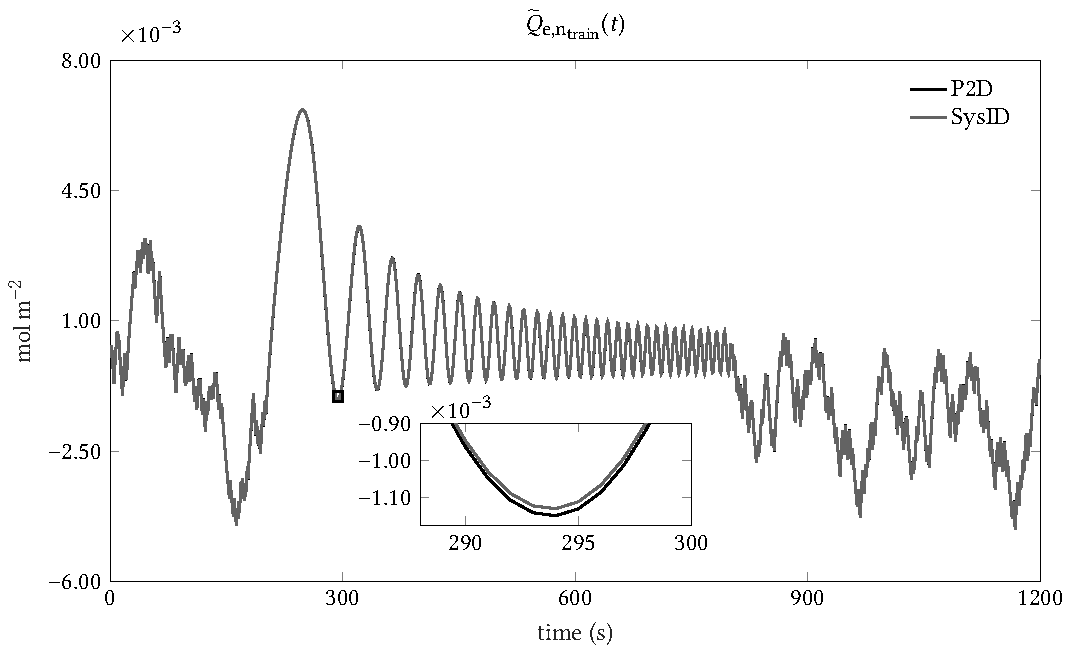
\includegraphics{p2d_sysid_train_qen.pdf}
    \caption[$\widetilde{Q}_{\text{e,n}}(t)$ outputs from \glsfmtshort{p2d} and
    identified transfer function for training profile]{%
        Time-evolution of~$\widetilde{Q}_{\text{e,n}}$ computed using the
        \glsfmtshort{p2d} model  and the identified transfer function
        of \cref{eq:finaldisctfneg} (scaled by~0.001) with the synthetic
        training input profile of \cref{fig:sysidtrainingcurrent}. The output
        predicted by the identified transfer function closely matches the `true'
        output obtained by a high-fidelity \glsfmtshort{p2d} simulation with an
        \glsfmtshort{rms} error of \SI{5.70e-6}{\mole\per\meter\squared} and a
        \glsfmtshort{mae} of~\SI{19.19e-6}{\mole\per\meter\squared}. Note that the
        transfer function in \cref{eq:finaldisctfneg} was originally obtained by
        scaling the output by~1000. The transfer function output is
        multiplied by the reciprocal of the same scaling factor to obtain the
        predicted response shown here, thereby once again justifying the
        linearity assumption for this subsystem.
    }%
    \label{fig:tfpredQentrain}
\end{figure}

\Cref{fig:tfpredQentrain} shows a comparison of the $\widetilde{Q}_{\text{e,n}}$
output for
\begin{enumerate*}[label=\emph{\alph*})]
    \item the \gls{p2d} model, and
    \item the identified transfer function of \cref{eq:finaldisctfneg}
\end{enumerate*}
using  the  training  current  profile  of \cref{fig:sysidtrainingcurrent}.  The
transfer function of \cref{eq:finaldisctfneg} was obtained by scaling the output
of the  training profile to  be of order~$\mathcal{O}(1)$  by a factor  of~1000.
Therefore,  for final  implementation and  comparison purposes,  the raw  output
produced  by applying  the transfer  function  needs to  be scaled  back by  its
reciprocal. If  the system  is linear,  then this scaling  factor shall  have no
impact  on  the  frequency-dependent  dynamics  of  the  subsystem.  The  output
predicted  by the  identified transfer  function is  virtually indistinguishable
from  the `true'  output computed  by post-processing  the \gls{p2d}  model with
an  \glsfmtshort{rms}  error   of  \SI{5.70e-6}{\mole\per\meter\squared}  and  a
\glsfmtshort{mae} of~\SI{19.19e-6}{\mole\per\meter\squared}.  This high accuracy
of the transfer  function prediction justifies the linearity  assumption for the
subsystem.  \Cref{fig:tfpredQepval}  presents  the  same  comparison  using  the
validation input profile for the subsystem in the positive electrode region. The
accuracy of  the identified transfer function  for this independent data  set is
clearly illustrated.

\begin{figure}[!htbp]
    \centering
    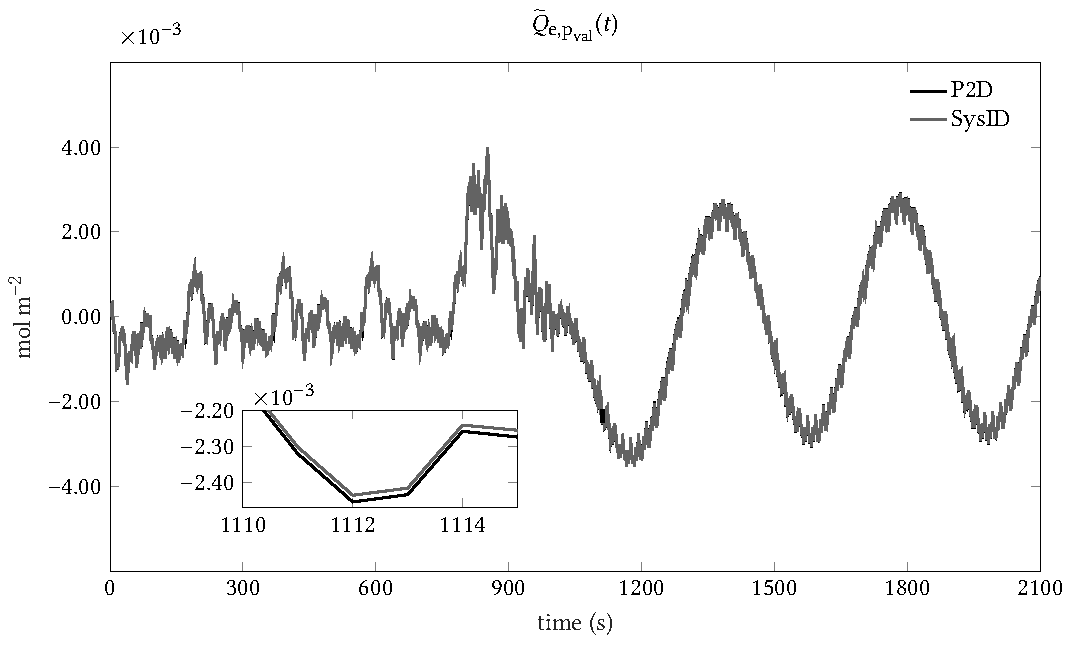
\includegraphics{p2d_sysid_val_qep.pdf}
    \caption[$\widetilde{Q}_{\text{e,p}}(t)$ outputs from \glsfmtshort{p2d} and
    identified transfer function for training profile]{%
        Time-evolution of~$\widetilde{Q}_{\text{e,p}}$ computed using the
        \glsfmtshort{p2d} model  and the identified transfer function
        of \cref{eq:finaldisctfpos} (scaled by~0.001) with the synthetic
        validation input profile of \cref{fig:sysidvalidationcurrent}. The output
        predicted by the identified transfer function closely matches the `true'
        output obtained by a high-fidelity \glsfmtshort{p2d} simulation with an
        \glsfmtshort{rms} error of \SI{12.07e-6}{\mole\per\meter\squared} and a
        \glsfmtshort{mae} of~\SI{31.59e-6}{\mole\per\meter\squared}. Note that the
        transfer function in \cref{eq:finaldisctfpos} was originally obtained by
        scaling the output by~1000. The transfer function output is
        multiplied by the reciprocal of the same scaling factor to obtain the
        predicted response shown here, thereby once again confirming the
        linearity of this subsystem.
    }%
    \label{fig:tfpredQepval}
\end{figure}

The  poles of \cref{eq:finaldisctfneg} are located at (0.9969, 0.9870, 0.9106,
0.6829) while those of  \cref{eq:finaldisctfpos} lie at (0.9967, 0.9880, 0.8952,
0.5842) on the Z-plane \ie{} close to each other. This  confirms  the hypothesis
that  the time-evolution subsystems  in these  two regions  exhibit similar
dynamics. The slight differences in  the pole locations could be attributed  to
the variations in  the  physical  parameters  pertaining  to the two  electrode
regions.  The numerator coefficients  of \cref{eq:finaldisctfneg} and
\cref{eq:finaldisctfpos} are  also  close  to  each other  except  that  their
signs  are  opposite  to each   other.  This   is to   be   expected,  since
as  seen   in  the   step response   plots   of \cref{fig:linearity},
$\widetilde{Q}_{\text{e,n}}$   and $\widetilde{Q}_{\text{e,p}}$ evolve in time
in opposite directions. This is also explained by  the fact  that, for  a given
applied current,  a decrease  in the number of ions in the negative electrode
has to be accompanied by an increase in the positive electrode and vice-versa
(the values of the changes are not exactly equal owing to the presence of the
separator). The identified transfer functions are thus consistent  and deemed to
be suitable for  representing the electrolyte time-evolution in these regions.

\subsection{Numerical implementation of identified transfer functions}\label{subsec:sysidnumericalimpl}

The concept  of deploying a Z-domain  transfer function may seem  incongruous to
the  one of  the  major  goals of  this  thesis \viz~time-domain  implementation
of  \glspl{rom} in  an  embedded  environment such  as  a  \gls{bms}. While  the
majority  of the  models is  derived  and implemented  entirely in  time-domain,
only  the two  time-evolution subsystems  of  the electrolyte  seems to  deviate
from  this  trajectory.  However,  an   explanation  for  this  is  provided  in
\cref{subsec:suitablesysid}.   In  particular,   it   was   mentioned  that   an
approximation-free  conversion   to  time-domain  from  Z-domain   exists,  that
mitigates this perceived drawback for  these two sub-systems. This conversion is
amenable for discrete-time implementation without any other modifications.

Starting from the generic structure of the identified transfer functions (see \cref{eq:outputwithsysonly}),

\begin{DispWithArrows}[fleqn,mathindent=0cm,jot=2ex,%
    ,xoffset=-4mm
    ]
    G(z) &= \frac{b_1z^{-1} + \dots + b_{n_b}z^{-{n_b}}}{1 + a_1z^{-1} + \dots + a_{n_a}z^{-{n_a}}} \Arrow{Replace with analogous \\ transfer operator $q=z$ \\ in time domain} \notag\\
    G(q) &= \frac{b_1q^{-1} + \dots + b_{n_b}q^{-{n_b}}}{1 + a_1q^{-1} + \dots + a_{n_a}q^{-{n_a}}} \Arrow{Apply the definition\\ of~$G(q)$ on the \glsfmtshort{lhs}}\notag \\
    \frac{y[k]}{u[k]} &= \frac{b_1q^{-1} + \dots + b_{n_b}q^{-{n_b}}}{1 + a_1q^{-1} + \dots + a_{n_a}q^{-{n_a}}} \Arrow{Cross-multiply}\notag \\
    \left(1 + a_1q^{-1} + \dots + a_{n_a}q^{-{n_a}}\right)y[k] &= \left(b_1q^{-1} + \dots + b_{n_b}q^{-{n_b}}\right)u[k] \Arrow{Expand on both sides} \notag \\
    y[k] + a_1q^{-1}y[k] + \dots + a_{n_a}q^{-{n_a}}y[k] &= b_1q^{-1}u[k] + \dots + b_{n_b}q^{-{n_b}}u[k] \Arrow{Apply the definition\\ $q^{-p}x[k] = x[k-p]$}\notag \\
    y[k] + a_1y[k-1] + \dots + a_{n_a}y[k-n_a] &= b_1u[k-1] + \dots + b_{n_b}u[k-n_b] \Arrow{Rearrange to obtain\\ the final expression}\notag \\
    y[k] &= -a_1y[k-1] - \dots - a_{n_a}y[k-n_a] \notag \\[-2ex]
         &\qquad   + b_1u[k-1] + \dots + b_{n_b}u[k-n_b] %\label{eq:lccde}
\end{DispWithArrows}

We  thus obtain  a  simple  algebraic expression  (a  difference equation)  that
computes the output  at the given time-step given past  inputs and outputs. This
is a highly memory-efficient implementation  since, at any given time-step, only
the previous~$n_a$ (four) output samples  and $n_b$ (four) input samples need to
be  `remembered'  (stored).  This  concludes all  the  aspects  (derivation  and
implementation) of  this author's new  model for the  electrolyte time-evolution
subsystem.  The  performance  of  this  model  for  computation  of  electrolyte
concentration needs to be evaluated, which is performed next.

